% Converted from part_a_measured_impacts.md by scripts/md_to_latex.py; edit this file.
% DRAFT v0.1 (2026-10-08). Part A of the paper: measured impacts on the road (three rides).
% Citations use Pandoc keys from ../references.bib, e.g. [@sensorlogger].
% Every number is taken from outputs/ or paper/figures/part_a_numbers.json (made by
% scripts/paper_part_a.py); sources are noted in HTML comments. Re-check them if any
% script is rerun. Individual recordings are reported in appendix_recordings.md.
% Decisions (2026-10-08): Part A uses all three recordings; combined results in the main
% text, per-recording results in the appendix; road bumps are not part of the paper.
% Table numbering: Part A uses Tables 1-3; Part B continues from Table~\ref{tab:4}.

\section{Measuring what riders experience on the road}\label{measuring-what-riders-experience-on-the-road}

\subsection{Data}\label{data}

\textbf{Rides.} One rider recorded three rides on Voi rental e-scooters in Oxford, ridden
legally within the national e-scooter trial \autocite{dft2024guidance,occ_trial}: one on
3 October 2026 (vehicle SZ22) and two on 7 October 2026 (vehicles UPAR and BTLZ). Voi
customer support confirmed that all three vehicles were Voiager 5 scooters
\autocite{voi2026support_rec01,voi2026support_rec0203}. The rides covered parts of Marston
Road, Morrell Avenue, Old Road (Headington), Headington Road and connecting streets.
Only the rider's own rides were recorded.

\textbf{Recording.} An iPhone 11 Pro Max was mounted on the handlebar and recorded with the
Sensor Logger app, version 1.67.1 \autocite{sensorlogger}. The app logged user acceleration
(gravity removed) and the gravity vector from the iOS sensor fusion
\autocite{apple_cmdevicemotion}, the raw accelerometer, the gyroscope (all at 100 Hz) and GPS
(about 1 Hz). The phone was set up before each ride and not touched while riding.

% outputs/recordings/<rec>/impact_stats.json; data/README.md

\begin{longtable}[]{@{}
  >{\raggedright\arraybackslash}p{(\linewidth - 10\tabcolsep) * \real{0.1667}}
  >{\raggedright\arraybackslash}p{(\linewidth - 10\tabcolsep) * \real{0.1667}}
  >{\raggedright\arraybackslash}p{(\linewidth - 10\tabcolsep) * \real{0.1667}}
  >{\raggedright\arraybackslash}p{(\linewidth - 10\tabcolsep) * \real{0.1667}}
  >{\raggedright\arraybackslash}p{(\linewidth - 10\tabcolsep) * \real{0.1667}}
  >{\raggedright\arraybackslash}p{(\linewidth - 10\tabcolsep) * \real{0.1667}}@{}}
\caption{The three rides. Riding time and distance count only travel at 7 km/h or faster (section 2.3).}\label{tab:1}\tabularnewline
\toprule\noalign{}
\begin{minipage}[b]{\linewidth}\raggedright
Ride
\end{minipage} & \begin{minipage}[b]{\linewidth}\raggedright
Date, start (local)
\end{minipage} & \begin{minipage}[b]{\linewidth}\raggedright
Vehicle (Voiager 5)
\end{minipage} & \begin{minipage}[b]{\linewidth}\raggedright
Recorded
\end{minipage} & \begin{minipage}[b]{\linewidth}\raggedright
Riding
\end{minipage} & \begin{minipage}[b]{\linewidth}\raggedright
Distance ridden
\end{minipage} \\
\midrule\noalign{}
\endfirsthead
\toprule\noalign{}
\begin{minipage}[b]{\linewidth}\raggedright
Ride
\end{minipage} & \begin{minipage}[b]{\linewidth}\raggedright
Date, start (local)
\end{minipage} & \begin{minipage}[b]{\linewidth}\raggedright
Vehicle (Voiager 5)
\end{minipage} & \begin{minipage}[b]{\linewidth}\raggedright
Recorded
\end{minipage} & \begin{minipage}[b]{\linewidth}\raggedright
Riding
\end{minipage} & \begin{minipage}[b]{\linewidth}\raggedright
Distance ridden
\end{minipage} \\
\midrule\noalign{}
\endhead
\bottomrule\noalign{}
\endlastfoot
1 & 3 Oct 2026, 18:30 & SZ22 & 13.7 min & 9.6 min & 2.89 km \\
2 & 7 Oct 2026, 10:37 & UPAR & 35.3 min & 5.9 min & 1.48 km \\
3 & 7 Oct 2026, 13:38 & BTLZ & 11.4 min & 6.3 min & 1.71 km \\
All & & & 60.4 min & 21.8 min & 6.08 km \\
\end{longtable}

Ride 2 also includes a walk after the rental ended and a long period with the phone at
rest; these parts are excluded from the impact analysis by the speed rule and were used
to check the recording method (section 2.2).

\subsection{Checking the recording method}\label{checking-the-recording-method}

Before using the phone data, we checked that they are internally sound and that riding
can be told apart from walking. The full method and results are given in Appendix B;
the main points are summarised here.

\textbf{Data quality.} In all three recordings the motion sensors ran at 99.72 Hz with
sampling intervals of 10.03 ms and no gaps, duplicated or out-of-order timestamps. During
the one period when the phone lay still (ride 2, after the walk), the acceleration noise
was about 0.001 g and the raw acceleration magnitude was 0.994 g, both small against the
1.0 g impact threshold used below. The phone's own estimate of GPS horizontal accuracy
had a median of 11--14 m per ride. These checks show internal consistency and
plausibility, not absolute accuracy, which would need a reference instrument.

% outputs/sensor_validity/quality_summary.csv

\textbf{Riding versus walking.} Walking and riding were distinguished with simple, fixed
rules on 4 s windows. The rules used established features: the vertical acceleration
obtained by projecting onto the gravity direction \autocite{mizell2003}; the share of its power
in the walking step band of 1.2--2.8 Hz, estimated with Welch's method \autocite{welch1967},
around measured mean step frequencies of 1.8--2.0 Hz \autocite{pachi2005}; the autocorrelation at
one step period, a measure of step regularity \autocite{moenilssen2004}; and GPS speed. Similar
signals are used for activity and transport-mode detection with phones
\autocite{kwapisz2011,reddy2010}; our aim was not a new classifier but a check that this app
and phone, mounted on a rental scooter, separate the two.

% outputs/sensor_validity/ground_truth_comparison.csv, walking_onsets.csv

In ride 2 the method found sustained walking from 10:46:47, the first step of a 275 s
walk at 2.04 steps per second (Figure~\ref{fig:1}). This agrees with two references, both with
one-minute precision: the Voi app recorded the rental ending at 10:46, and the rider
recalled walking ``after 10 minutes'' of the recording (10:47). In rides 1 and 3, which
the rider confirmed contained no walking, no walking bout was detected; isolated
walking labels covered 6 s and 8 s, all after the ride had ended. In 1,126 windows where
GPS alone showed riding speed (12 km/h or more), none met the walking criteria. With one
walking episode this shows that the data separate riding from walking; it does not give
a detection rate.

\begin{figure}
\centering
{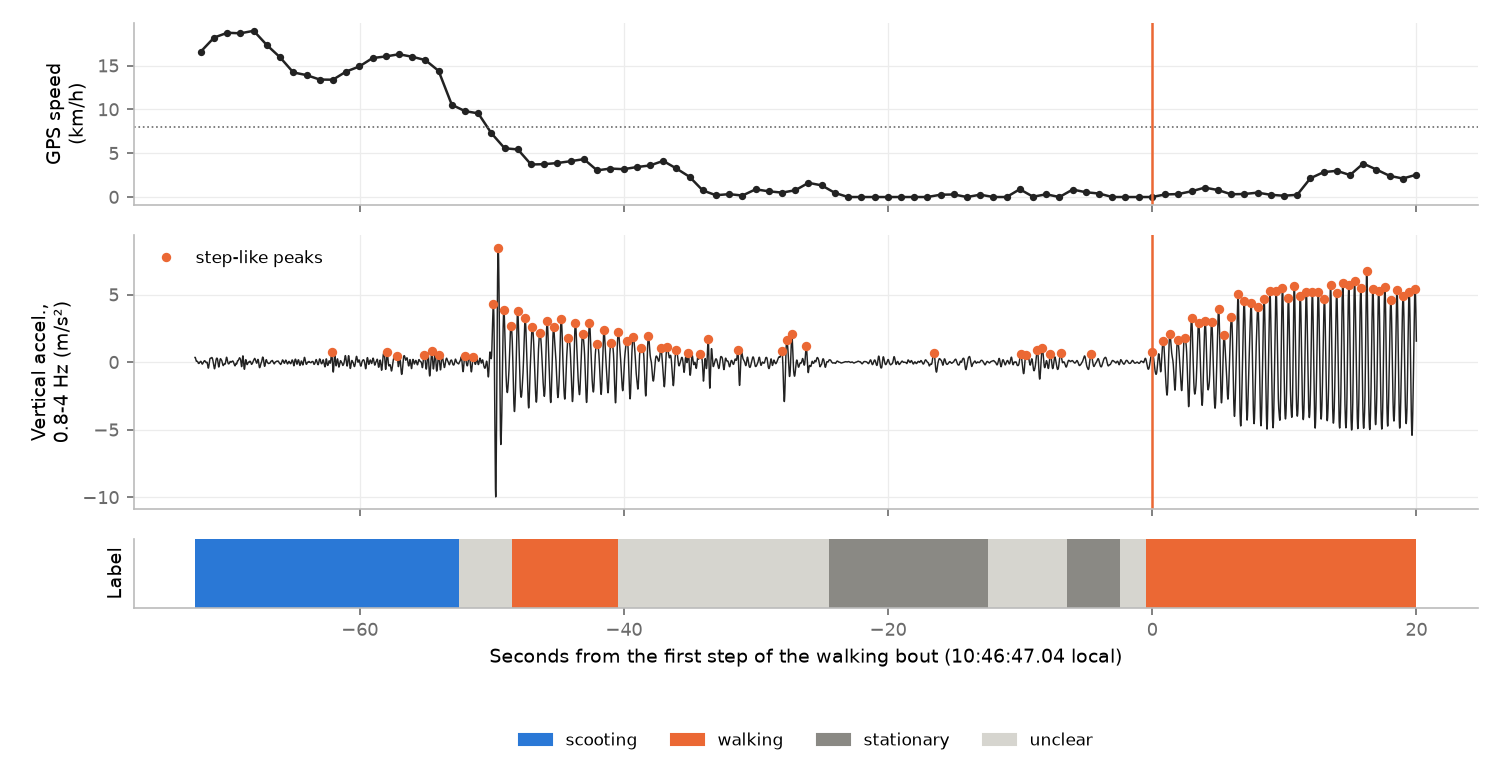
\includegraphics[width=\linewidth]{fig_a1_walk_onset.png}}
\caption{Transition from riding to walking in ride 2. Top: GPS speed; middle: vertical
acceleration (0.8--4 Hz) with step-like peaks; bottom: labels from the window rules. Time
0 is the first step of sustained walking (10:46:47). GPS speed rose only about 12 s after
walking began.}\label{fig:1}
\end{figure}

\textbf{Implications for impact detection.} Two findings bear on the method in section 2.3.
First, walking alone produced 11 peaks of 1.0 g or more (maximum 1.19 g) in ride 2's
walk; the speed rule excluded all of them, and all impacts in ride 2 occurred during
the ride. Second, the GPS-reported speed under-read walking: 3.0 km/h against at least
4.6 km/h from the GPS positions themselves. It was also below the position-based lower
bound in 4 of 6 riding segments, by 0.2--3.2 km/h. Because the speed rule uses the
reported speed, some impacts at low riding speeds may have been excluded; this was not
quantified. Dedicated GPS receivers have also been found to underestimate speed on
curved paths \autocite{witte2004}.

\subsection{Impact detection}\label{impact-detection}

% scripts/impact_map.py; outputs/recordings/<rec>/impacts_params.json

The user acceleration was projected sample by sample onto the upward direction given by
the gravity vector, so that the result does not depend on how the phone sat in its
mount \autocite{mizell2003}. An \textbf{impact} is a peak in the absolute vertical acceleration of at
least \textbf{1.0 g}, at least 0.5 s after the previous one (SciPy \texttt{find\_peaks}
\autocite{virtanen2020scipy}), while the GPS-reported speed was at least \textbf{7 km/h}. The speed
rule excludes getting on and off, stops, walking and handling the phone. Each impact
was located by interpolating the GPS track, using only fixes with a reported accuracy
of 20 m or better. For each impact, the rotation rate of the handlebar (gyroscope) in
the 1.5 s after the impact was divided by that in the 2 s before it; a ratio of 1.5 or
more is reported as \textbf{marked wobble}.

The 1.0 g threshold, the 7 km/h speed rule and the 1.5 wobble ratio are analyst
choices, not established criteria. A fixed threshold in g was used, rather than one set
per ride, so that rides and vehicles can be compared directly.

\subsection{Roads and repeated spots}\label{roads-and-repeated-spots}

% scripts/impact_report.py, scripts/combined_outputs.py, scripts/spot_links.py

Each impact and each second of riding was assigned to a study road if it lay within 20 m
of the road's centreline in OpenStreetMap \autocite{osm,overpass}, and to ``other roads''
otherwise. Rates per km are given only where at least 0.2 km was ridden on a road (an
analyst choice; shorter distances give meaningless rates).

To find places that produce impacts repeatedly, the impacts of all three rides were
pooled and grouped by single-linkage clustering \autocite{sibson1973} with a 30 m distance,
which is larger than the typical GPS error. Each group is a \textbf{spot}, ranked in three
tiers: impacts from two or more separate rides (tier 1), two or more impacts from one
ride (tier 2), and single impacts (tier 3). The rides share one rider, phone and route,
so repeated hits on a spot are repeated measurements of one place, not independent
confirmations.

\subsection{Comparison with FixMyStreet}\label{comparison-with-fixmystreet}

% scripts/fms_compare.py; data/fixmystreet/reports_<rec>.bbox.json

Public road-surface reports were taken from FixMyStreet \autocite{fixmystreet} for each ride's
own area (potholes, carriageway defects, manholes and drain ironwork; reports in two
catch-all categories were kept only if their title described the road surface). An
impact counts as near a report if a report made in the 365 days before that ride lies
within 25 m. Because reports are dense, each rate is compared with a \textbf{route
baseline}: the share of all points along the ridden route that lie within 25 m of
such a report, which is what chance alone would give. With reports from all years
instead of the last 365 days, 70--87\% of route points lie near a report, which is
why only recent reports are used.

\subsection{Results}\label{results}

\subsubsection{Impacts}\label{impacts}

% paper/figures/part_a_numbers.json: per_ride_and_pooled, pooled

The three rides produced \textbf{100 impacts} over 6.08 km of riding, 16.4 per km, or one
every 61 m (Table~\ref{tab:2}). Their median peak was 1.27 g (interquartile range 1.13--1.73 g);
32 reached 1.5 g, 12 reached 2.0 g, and 95\% were at or below 2.68 g (Figure~\ref{fig:2}). One impact,
in ride 3, reached 6.28 g; all others were 2.97 g or less. Thirty-two impacts were
followed by marked wobble, 12 of them also at 1.5 g or more.

\begin{longtable}[]{@{}
  >{\raggedright\arraybackslash}p{(\linewidth - 14\tabcolsep) * \real{0.1250}}
  >{\raggedright\arraybackslash}p{(\linewidth - 14\tabcolsep) * \real{0.1250}}
  >{\raggedright\arraybackslash}p{(\linewidth - 14\tabcolsep) * \real{0.1250}}
  >{\raggedright\arraybackslash}p{(\linewidth - 14\tabcolsep) * \real{0.1250}}
  >{\raggedright\arraybackslash}p{(\linewidth - 14\tabcolsep) * \real{0.1250}}
  >{\raggedright\arraybackslash}p{(\linewidth - 14\tabcolsep) * \real{0.1250}}
  >{\raggedright\arraybackslash}p{(\linewidth - 14\tabcolsep) * \real{0.1250}}
  >{\raggedright\arraybackslash}p{(\linewidth - 14\tabcolsep) * \real{0.1250}}@{}}
\caption{Impacts per ride and pooled. Pooled values describe the three rides together; the rides are not independent samples.}\label{tab:2}\tabularnewline
\toprule\noalign{}
\begin{minipage}[b]{\linewidth}\raggedright
Ride
\end{minipage} & \begin{minipage}[b]{\linewidth}\raggedright
Impacts
\end{minipage} & \begin{minipage}[b]{\linewidth}\raggedright
Per km
\end{minipage} & \begin{minipage}[b]{\linewidth}\raggedright
Median (g)
\end{minipage} & \begin{minipage}[b]{\linewidth}\raggedright
Max (g)
\end{minipage} & \begin{minipage}[b]{\linewidth}\raggedright
≥ 1.5 g
\end{minipage} & \begin{minipage}[b]{\linewidth}\raggedright
≥ 2.0 g
\end{minipage} & \begin{minipage}[b]{\linewidth}\raggedright
Marked wobble
\end{minipage} \\
\midrule\noalign{}
\endfirsthead
\toprule\noalign{}
\begin{minipage}[b]{\linewidth}\raggedright
Ride
\end{minipage} & \begin{minipage}[b]{\linewidth}\raggedright
Impacts
\end{minipage} & \begin{minipage}[b]{\linewidth}\raggedright
Per km
\end{minipage} & \begin{minipage}[b]{\linewidth}\raggedright
Median (g)
\end{minipage} & \begin{minipage}[b]{\linewidth}\raggedright
Max (g)
\end{minipage} & \begin{minipage}[b]{\linewidth}\raggedright
≥ 1.5 g
\end{minipage} & \begin{minipage}[b]{\linewidth}\raggedright
≥ 2.0 g
\end{minipage} & \begin{minipage}[b]{\linewidth}\raggedright
Marked wobble
\end{minipage} \\
\midrule\noalign{}
\endhead
\bottomrule\noalign{}
\endlastfoot
1 & 40 & 13.8 & 1.19 & 2.80 & 6 & 4 & 13 \\
2 & 39 & 26.4 & 1.34 & 2.87 & 15 & 3 & 11 \\
3 & 21 & 12.3 & 1.67 & 6.28 & 11 & 5 & 8 \\
All & 100 & 16.4 & 1.27 & 6.28 & 32 & 12 & 32 \\
\end{longtable}

\begin{figure}
\centering
{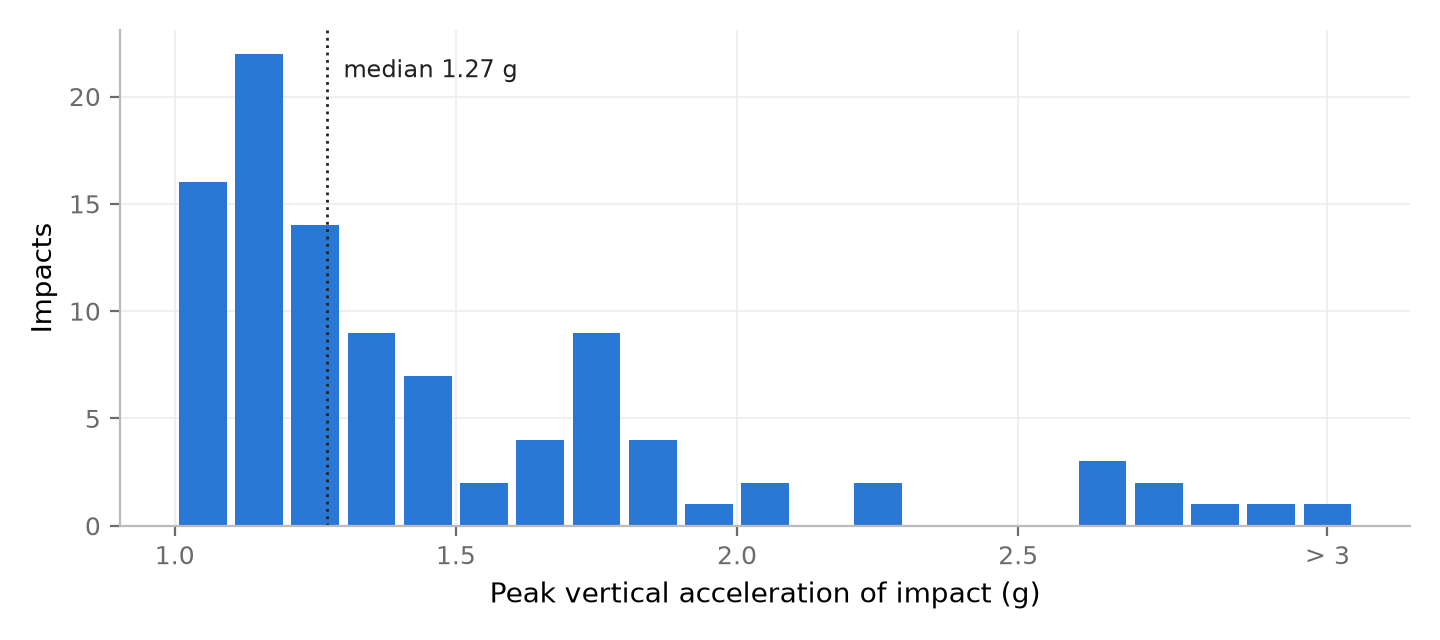
\includegraphics[width=\linewidth]{fig_a2_severity.png}}
\caption{Peak vertical acceleration of the 100 impacts from all three rides. The
detection threshold is 1.0 g; impacts above 3 g are shown as one bar
(one impact, 6.28 g).}\label{fig:2}
\end{figure}

Rates differed between rides (12.3--26.4 per km). Ride 2's higher rate comes largely
from one stretch where 13 impacts followed each other every 0.6--1.2 s at about 8 km/h
over roughly 20 m; ride 3 also produced a cluster there (spot P3, Table~\ref{tab:3}). Whether
this is a rough surface, such as setts or a broken patch, has not yet been checked.

\textbf{Speed and severity.} In ride 1 the impact peak was not related to speed (Spearman
ρ = 0.03, p = 0.88 \autocite{spearman1904}). In rides 2 and 3, slower impacts were stronger
(ρ = −0.63 and −0.68), and pooled ρ = −0.48. This pooled association comes mostly from
the two dense clusters at about 8 km/h (Figure~\ref{fig:speed}): without the spots of 10
or more impacts, ρ = −0.12 (p = 0.33, n = 71), and with one value per spot, ρ = −0.36
(p = 0.04, n = 33). Because impacts within a spot are not independent, these p-values
overstate the evidence; no conclusion about speed is drawn.

% paper/figures/fig_a5_speed.png (scripts/paper_part_a.py, fig_speed)
\begin{figure}
\centering
{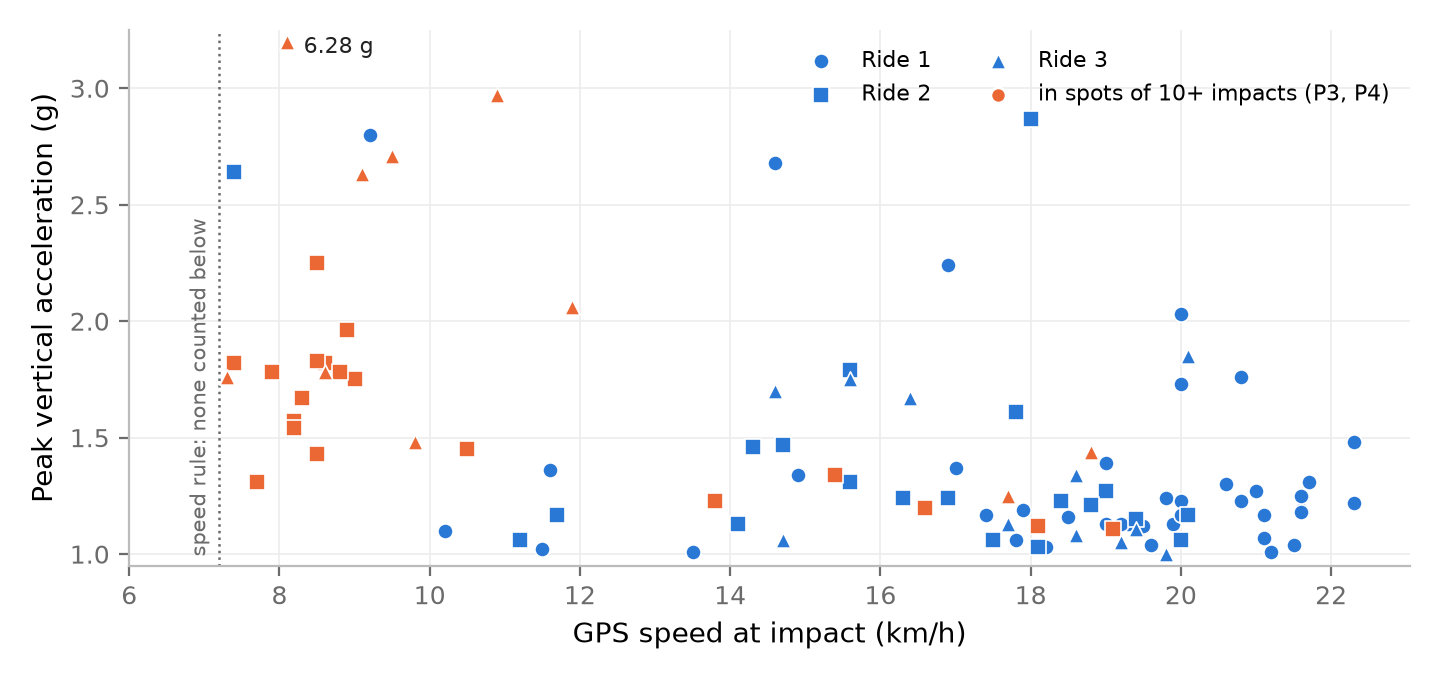
\includegraphics[width=\linewidth]{fig_a5_speed.png}}
\caption{GPS speed at impact against peak vertical acceleration, all 100 impacts (marker
shape: ride). Orange: the 29 impacts in the two spots with 10 or more impacts (P3, P4,
Table~\ref{tab:3}), which produce most of the pooled speed--severity association. The
6.28 g impact is drawn at the top edge. Dotted line: speed rule (7.2 km/h); impacts at
lower speeds are not counted.}\label{fig:speed}
\end{figure}

\subsubsection{Where the impacts were}\label{where-the-impacts-were}

% outputs/combined/by_road.csv

Per km ridden, the study roads gave 12.3 impacts (Marston Road, 2.52 km), 14.3 (Morrell
Avenue, 1.05 km) and 8.3 (Old Road, 0.24 km), and other roads 22.7 (2.25 km)
(Figure~\ref{fig:3}). Headington Road was ridden for only 0.02 km, too little for a rate.

\begin{figure}
\centering
{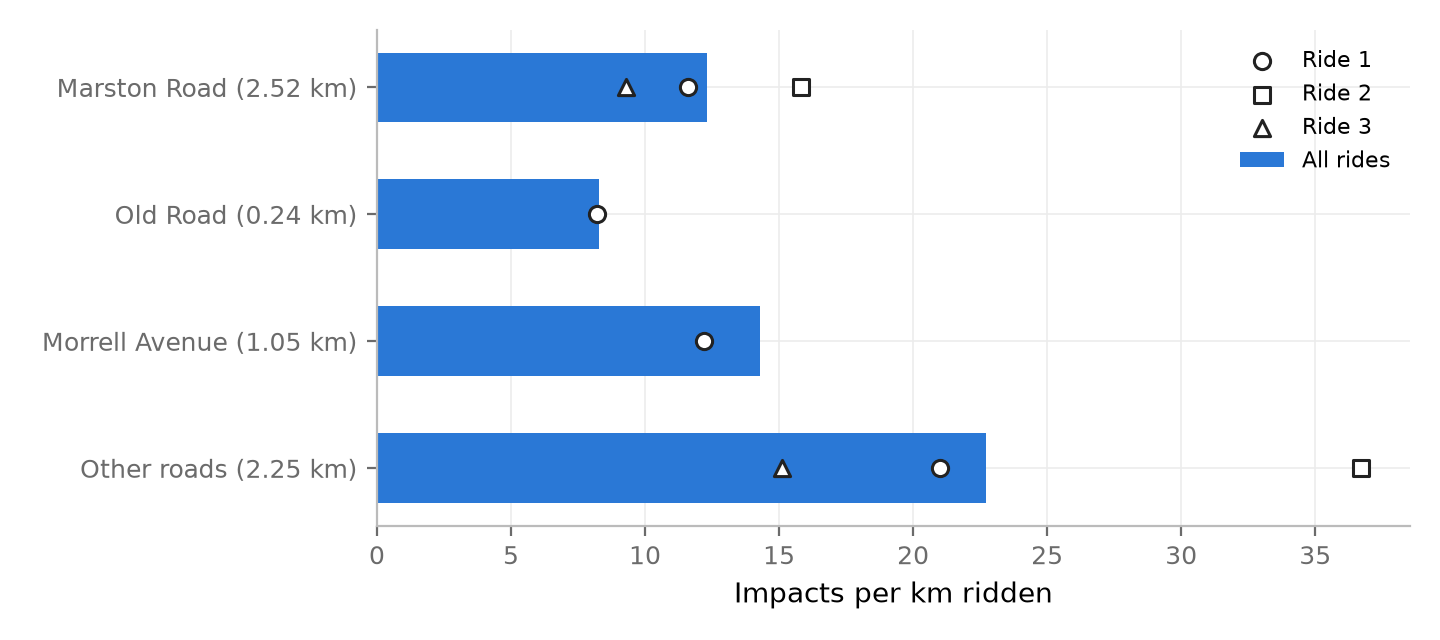
\includegraphics[width=\linewidth]{fig_a3_roads.png}}
\caption{Impacts per km ridden by road, all rides (bars) and per ride (markers).
Rates are shown only where at least 0.2 km was ridden on the road by that ride; the
distance ridden on each road over all rides is given in brackets.}\label{fig:3}
\end{figure}

% outputs/combined/spot_links.csv; part_a_numbers.json: spots

The impacts formed 33 spots: \textbf{10 hit on two or more separate rides}, 10 with several
impacts from one ride, and 13 single impacts (Figure~\ref{fig:4}). Two spots on Marston Road, P1
and P2, were hit on all three rides (Table~\ref{tab:3}). The strongest single impact, 6.28 g, lies
in spot P4, which was hit on two rides.

\begin{figure}
\centering
{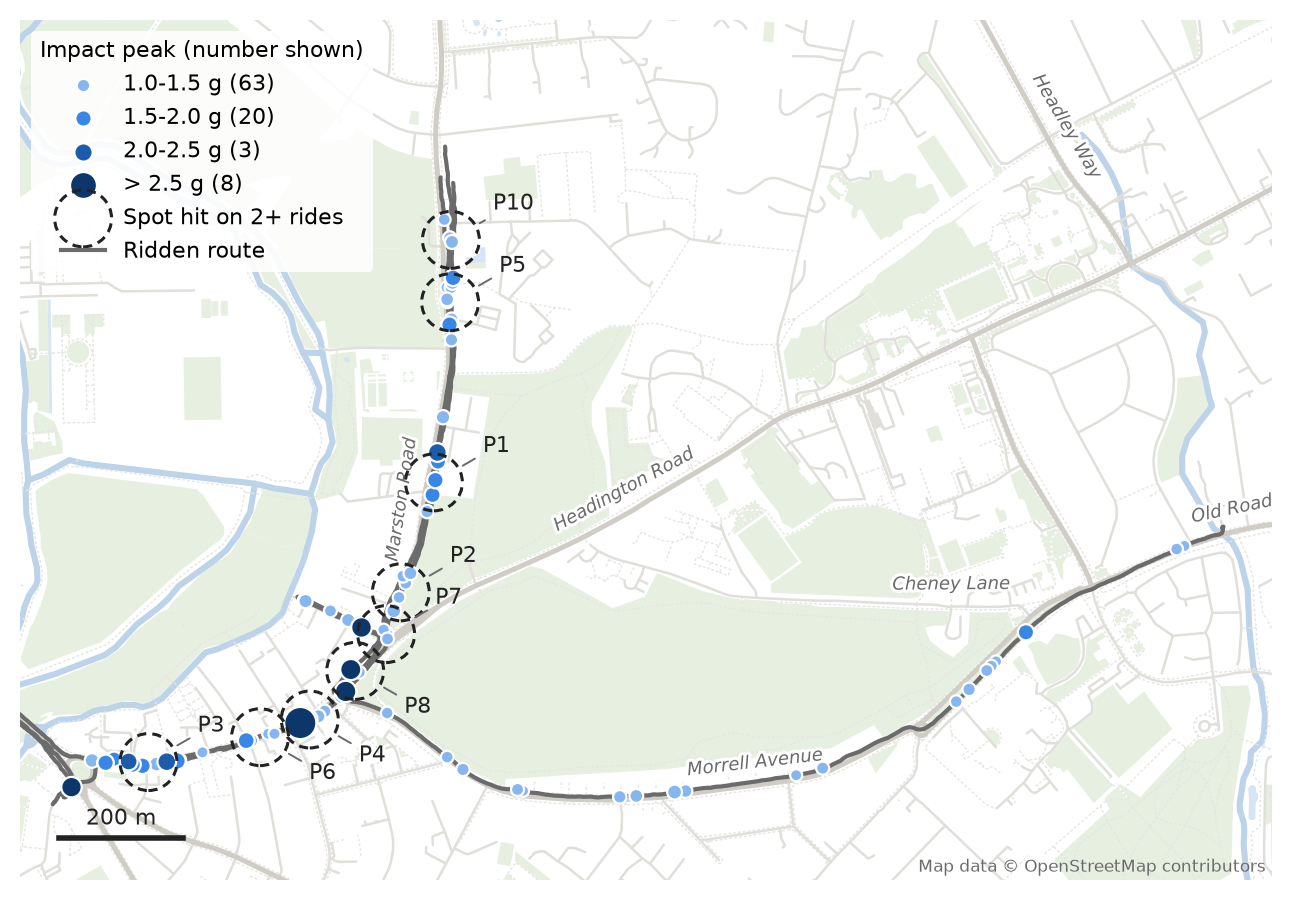
\includegraphics[width=\linewidth]{fig_a4_map.png}}
\caption{Impacts from all three rides on the ridden routes, coloured and sized by peak
vertical acceleration; dashed circles mark the 10 spots hit on two or more rides
(Table~\ref{tab:3}). For privacy, the first and last 200 m of each route are not drawn; the 6
impacts in those parts are included in all statistics. Background: streets, paths, parks and
water from OpenStreetMap \autocite{osm}, map data \textcopyright{} OpenStreetMap contributors (ODbL).}\label{fig:4}
\end{figure}

\begin{longtable}[]{@{}
  >{\raggedright\arraybackslash}p{(\linewidth - 12\tabcolsep) * \real{0.1429}}
  >{\raggedright\arraybackslash}p{(\linewidth - 12\tabcolsep) * \real{0.1429}}
  >{\raggedright\arraybackslash}p{(\linewidth - 12\tabcolsep) * \real{0.1429}}
  >{\raggedright\arraybackslash}p{(\linewidth - 12\tabcolsep) * \real{0.1429}}
  >{\raggedright\arraybackslash}p{(\linewidth - 12\tabcolsep) * \real{0.1429}}
  >{\raggedright\arraybackslash}p{(\linewidth - 12\tabcolsep) * \real{0.1429}}
  >{\raggedright\arraybackslash}p{(\linewidth - 12\tabcolsep) * \real{0.1429}}@{}}
\caption{Spots hit on two or more rides, with the nearest FixMyStreet road-surface report made in the 365 days before the ride.}\label{tab:3}\tabularnewline
\toprule\noalign{}
\begin{minipage}[b]{\linewidth}\raggedright
Spot
\end{minipage} & \begin{minipage}[b]{\linewidth}\raggedright
Rides
\end{minipage} & \begin{minipage}[b]{\linewidth}\raggedright
Impacts
\end{minipage} & \begin{minipage}[b]{\linewidth}\raggedright
Max (g)
\end{minipage} & \begin{minipage}[b]{\linewidth}\raggedright
Road
\end{minipage} & \begin{minipage}[b]{\linewidth}\raggedright
Recent report within 25 m
\end{minipage} & \begin{minipage}[b]{\linewidth}\raggedright
Nearest recent report
\end{minipage} \\
\midrule\noalign{}
\endfirsthead
\toprule\noalign{}
\begin{minipage}[b]{\linewidth}\raggedright
Spot
\end{minipage} & \begin{minipage}[b]{\linewidth}\raggedright
Rides
\end{minipage} & \begin{minipage}[b]{\linewidth}\raggedright
Impacts
\end{minipage} & \begin{minipage}[b]{\linewidth}\raggedright
Max (g)
\end{minipage} & \begin{minipage}[b]{\linewidth}\raggedright
Road
\end{minipage} & \begin{minipage}[b]{\linewidth}\raggedright
Recent report within 25 m
\end{minipage} & \begin{minipage}[b]{\linewidth}\raggedright
Nearest recent report
\end{minipage} \\
\midrule\noalign{}
\endhead
\bottomrule\noalign{}
\endlastfoot
P1 & 3 & 6 & 2.24 & Marston Road & No & 60 m (closed) \\
P2 & 3 & 6 & 1.47 & Marston Road & No & 44 m (closed) \\
P3 & 2 & 19 & 2.25 & Other & Yes & 5 m (closed) \\
P4 & 2 & 10 & 6.28 & Other & Yes & 8 m (fixed) \\
P5 & 2 & 9 & 1.79 & Marston Road & No & 121 m (closed) \\
P6 & 2 & 4 & 1.85 & Other & Yes & 8 m (closed) \\
P7 & 2 & 3 & 1.17 & Marston Road & Yes & 8 m (closed) \\
P8 & 2 & 2 & 2.80 & Other & No & 38 m (closed) \\
P9 & 2 & 2 & 2.03 & Marston Road & No & 125 m (fixed) \\
P10 & 2 & 2 & 1.34 & Marston Road & No & 87 m (closed) \\
\end{longtable}

\subsubsection{Comparison with FixMyStreet}\label{comparison-with-fixmystreet-1}

% outputs/recordings/<rec>/fms_match_rates.csv

At the level of single impacts, FixMyStreet reports did not single out the places where
impacts occurred. A recent report lay within 25 m of 2 of 40 impacts in ride 1 (5\%,
route baseline 14\%), 12 of 39 in ride 2 (31\%, baseline 33\%) and 9 of 21 in ride 3
(43\%, baseline 34\%): close to what chance would give in each ride. At the level of
spots, 6 of the 10 spots hit on two or more rides had no recent report within 25 m,
including both spots hit on all three rides (Table~\ref{tab:3}). Spot P4, with the 6.28 g impact,
had a report within 8 m marked ``fixed''; its report and repair dates have not been
checked. A missing FixMyStreet report does not mean that a defect was unknown to the
highway authority, which also receives reports through other channels and inspects
roads itself.

\textbf{Visual check.} The spots are being checked in street-level imagery with rules fixed
in advance (Appendix C); results are pending.

% TODO: fill in from outputs/combined/spot_links.csv (imagery_date, what_visible)

\subsubsection{Summary of Part A}\label{summary-of-part-a}

Riding three Voiager 5 scooters over 6.08 km produced 100 jolts of 1 g or more at the
handlebar, about one every 61 m, a third of them 1.5 g or more. Ten places produced
impacts on two or more separate rides, and most of these had no recent public report.
These results come from one rider, one phone and short routes, and use analyst-chosen
thresholds; they describe exposure on these rides, not the risk to riders in general.
